	
	\subsection*{1.}
	
	Au départ, il y a 6 jetons rouges sur 10, donc \(p(R_1) = \dfrac{6}{10} = \dfrac{3}{5} = 0,6\).
	
	Si un jeton rouge a été tiré, il reste 5 rouges sur 9 jetons, donc \(p_{R_1}(R_2) = \dfrac{5}{9}\).
	
	Si un jeton noir a été tiré en premier, il reste 6 rouges sur 9 jetons, donc \(p_{\overline{R_1}}(R_2) = \dfrac{6}{9} = \dfrac{2}{3}\).
	
	\begin{center}
		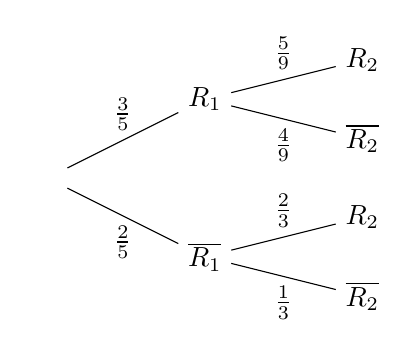
\begin{tikzpicture}
			\node (P_-1_0) at (-2,-1.5) {$\phantom{A}$};
			\node (P_0_0) at (0,-0.5) {$R_1$};
			\draw (P_-1_0) -- (P_0_0) node[midway, above] {$\frac35$};
			\node (P_1_0) at (2,-0) {$R_2$};
			\draw (P_0_0) -- (P_1_0) node[midway, above] {$\frac59$};
			\node (P_1_1) at (2,-1) {$\overline{R_2}$};
			\draw (P_0_0) -- (P_1_1) node[midway, below] {$\frac49$};
			\node (P_0_2) at (0,-2.5) {$\overline{R_1}$};
			\draw (P_-1_0) -- (P_0_2) node[midway, below] {$\frac25$};
			\node (P_1_2) at (2,-2) {$R_2$};
			\draw (P_0_2) -- (P_1_2) node[midway, above] {$\frac23$};
			\node (P_1_3) at (2,-3) {$\overline{R_2}$};
			\draw (P_0_2) -- (P_1_3) node[midway, below] {$\frac13$};
		\end{tikzpicture}
	\end{center}
	
	\subsection*{2.}
	
	\subsubsection*{a.}
	
	On a \(p(A) = p(R_1 \cap R_2) = p(R_1) \times p_{R_1}(R_2) = \dfrac{3}{5} \times \dfrac{5}{9} = \dfrac{3}{9} = \dfrac{1}{3}\).
	
	\subsubsection*{b.}
	
	L'évènement \(\overline{A}\) signifie \(\text{\guillemotleft{} le joueur obtient au plus un jeton rouge \guillemotright{}}\).
	
	\subsubsection*{c.}
	
	On a \(p(\overline{R_1} \cap R_2) = p(\overline{R_1}) \times p_{\overline{R_1}}(R_2) = \dfrac{2}{5} \times \dfrac{2}{3} = \dfrac{4}{15}\).
	
	D'après la loi des probabilités totales :
	\[
	p(R_2) = p(R_1 \cap R_2) + p(\overline{R_1} \cap R_2) = \dfrac{1}{3} + \dfrac{4}{15} = \dfrac{5}{15} + \dfrac{4}{15} = \dfrac{9}{15} = \dfrac{3}{5} = 0,6.
	\]
	
	\subsubsection*{d.}
	
	On a \(p_{\overline{R_2}}(R_1) = \dfrac{p(\overline{R_2} \cap R_1)}{p(R_2)} = \dfrac{p(R_1 \cap \overline{R_2})}{p(R_2)} = \dfrac{\dfrac{3}{5} \times \dfrac{4}{9}}{\dfrac{3}{5}} = \dfrac{4}{9} < \dfrac{4,5}{9} = 0,5\).\\
	 L'affirmation est donc fausse.
	
